%% Template for INT1414 reports
%% by Thanh Le
%% based on LaTeX work of Robin Turner.
%% Adapted from the IEEE peer review template


\documentclass[conference]{IEEEtran}
\IEEEoverridecommandlockouts
%\usepackage{cite} % Tidies up citation numbers.
\usepackage{url} % Provides better formatting of URLs.
\usepackage{booktabs} % Allows the use of \toprule, \midrule and \bottomrule in tables for horizontal lines
\usepackage{graphicx}
%my package
%\usepackage[vietnamese]{babel}
\usepackage{listings}

\hyphenation{op-tical net-works semi-conduc-tor} % Corrects some bad hyphenation 

% The preceding line is only needed to identify funding in the first footnote. If that is unneeded, please comment it out.
\usepackage{amsmath,amssymb,amsfonts}
\usepackage{algorithmic}
\usepackage{textcomp}
\usepackage{xcolor}
\def\BibTeX{{\rm B\kern-.05em{\sc i\kern-.025em b}\kern-.08em
    T\kern-.1667em\lower.7ex\hbox{E}\kern-.125emX}}


\begin{document}
% can use linebreaks \\ within to get better formatting as desired
\title{Chiến lược nhất quán trong cơ sở dữ liệu phân tán:\\ CAP Theorem và các giải pháp thực tế}


% author names and affiliations
\author{\IEEEauthorblockN{ T. V. Đinh}
\IEEEauthorblockA{\textit{Khoa Công Nghệ Thông Tin 2} \\
\textit{Học viện Công nghệ Bưu chính Viễn thông cơ sở tại TP.Hồ Chí Minh}\\
D20CQCNHT01-N \\
email: n20dccn070@student.ptithcm.edu.vn}}
% \author{A. V. Nguyen \\
% Department of Information Technology 2\\
% Posts and Telecommunications Institute of Technology at HCM city\\
% Class\\
% email:
% }
\date{25/4/15}

% make the title area
\maketitle
% \IEEEpeerreviewmaketitle
\begin{abstract}
    
Trong bối cảnh hệ thống phân tán ngày càng phổ biến, việc lựa chọn chiến lược đảm bảo tính nhất quán dữ liệu là một thách thức lớn đối với các kỹ sư hệ thống. Bài nghiên cứu này giới thiệu định lý CAP và phân tích chi tiết các chiến lược nhất quán được triển khai trong bốn hệ quản trị cơ sở dữ liệu phân tán hiện đại: Amazon DynamoDB, Apache Cassandra, MongoDB và Google Spanner. Mỗi hệ thống được đánh giá dựa trên kiến trúc tổng thể, cơ chế đảm bảo nhất quán và khả năng chịu lỗi, từ đó làm rõ sự đánh đổi giữa ba yếu tố trong định lý CAP: tính nhất quán (Consistency), tính sẵn sàng (Availability) và dung sai phân vùng (Partition Tolerance).

\end{abstract}

\section{Giới thiệu}
Trong kỷ nguyên của điện toán đám mây và các ứng dụng phân tán, cơ sở dữ liệu phân tán đóng vai trò then chốt trong việc đảm bảo hiệu suất, khả năng mở rộng và độ tin cậy của hệ thống. Những dịch vụ như mạng xã hội, hệ thống thương mại điện tử đòi hỏi phải lưu trữ và xử lý lượng lớn dữ liệu theo thời gian thực, đồng thời đảm bảo dữ liệu luôn sẵn sàng và nhất quán cho người dùng ở nhiều khu vực khác nhau. 

Tuy nhiên, thiết kế một hệ cơ sở dữ liệu phân tán luôn đối mặt với những mâu thuẫn nội tại giữa các tính chất: tính sẵn sàng, tính nhất quán, khả năng chịu lỗi phân vùng. Sự đánh đổi giữa ba tính chất này đã được biết đến vào năm 1985 bởi Susan, Hector và Dale \cite{davidson}. Sau đó được phát biểu bởi Eric Brewer \cite{brewer} và được chứng minh bởi Gilbert và Lynch, và khi này chính thức được gọi tên là định lý CAP \cite{gilbert}. Điều này buộc các hệ thống phải đưa ra sự đánh đổi nhất định.
\begin{figure}[h]
    \centering
    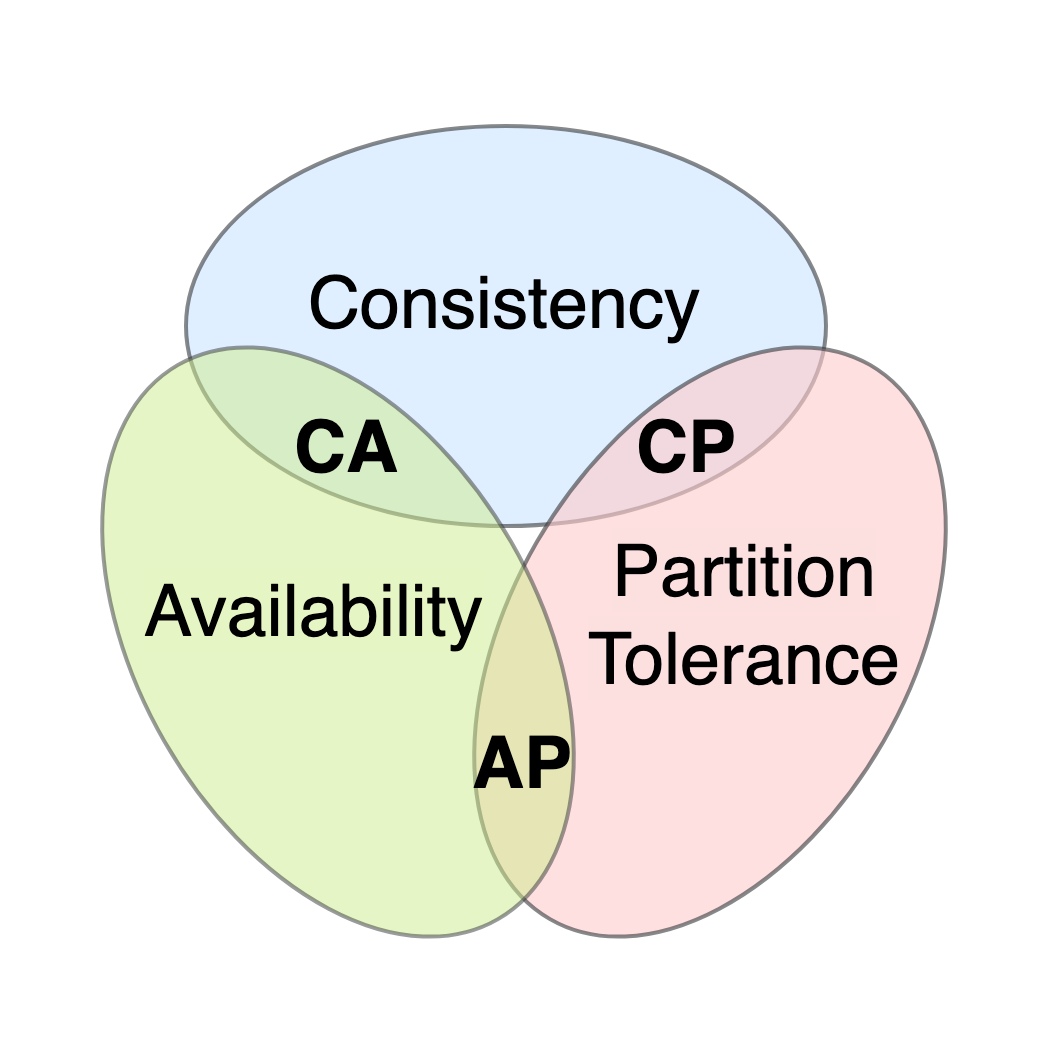
\includegraphics[width=0.5\linewidth]{pic/CAP_Theorem_Venn_Diagram.png}
    \caption{Lược đồ VEN mô tả định lý CAP}
    \label{fig:ven}
\end{figure}

Nhiều giải pháp có thể kể đến như: Amazon DynamoDB, Apache Cassandra, MongoDB hay Google Spanner đã phát triển các chiến lược nhất quán khác nhau để cân bằng các yếu tố trên. Việc hiểu rõ cách thức triển khai và đánh đổi trong từng hệ thống không chỉ hỗ trợ việc lựa chọn nền tảng phù hợp, mà còn định hướng cho thiết kế kiến trúc phân tán hiệu quả hơn.
\section{Xác định vấn đề}   
Với sự gia tăng nhanh chóng của các hệ thống phân tán quy mô lớn, việc đảm bảo tính toàn vẹn và nhất quán của dữ liệu trong môi trường mạng không ổn định trở thành một thách thức lớn. Các ứng dụng như ngân hàng trực tuyến, thương mại điện tử hay mạng xã hội đòi hỏi cơ sở dữ liệu phải duy trì tính đúng của thông tin trong khi vẫn đáp ứng yêu cầu về tính sẵn sàng.

Định lý CAP khẳng định rằng khi có phân vùng mạng thì một hệ thống phân tán buộc phải hy sinh một trong hai thuộc tính: tính sẵn sàng hoặc tính nhất quán. Do đó, bài nghiên cứu tập trung vào:
\begin{itemize}
    \item Giới thiệu định lý CAP.
    \item Xác định và so sánh các chiến lược nhất quán được áp dụng trong các hệ cơ sở dữ liệu phân tán phổ biến (DynamoDB, Cassandra, MongoDB, Spanner).
    \item Phân tích các đánh đổi về độ trễ và khả năng mở rộng khi lựa chọn mỗi chiến lược.
\end{itemize}


\section{Phương pháp luận}
Bài nghiên cứu này sử dụng phương pháp phân tích tài liệu, kết hợp với phương pháp so sánh định tính và định lượng các hệ cơ sở dữ liệu phân tán phổ biến. Tài liệu được khảo sát bao gồm các bài báo khoa học, tài liệu kỹ thuật, sách và hướng dẫn chính thức từ nhà phát triển.
Quá trình nghiên cứu được thực hiện theo các bước:
\begin{itemize}
\item Tổng hợp cơ sở lý thuyết: Thu thập thông tin từ các nghiên cứu liên quan đến định lý CAP, mô hình nhất quán của các hệ quản trị cơ sở dữ liệu phân tán.
\item Phân tích hệ thống cụ thể: Đánh giá chi tiết kiến trúc, cơ chế đồng bộ, giao thức replication, chiến lược đọc ghi và cách hệ thống xử lý phân vùng mạng.
\item Đánh giá các hệ thống theo tiêu chí chuẩn: mức độ nhất quán, độ trễ truy vấn, khả năng mở rộng.
\end{itemize}

\section{Định nghĩa định lý CAP}
Định lý CAP là một nguyên lý nền tảng trong thiết kế và phân tích các hệ thống phân tán. Về cơ bản, định lý này khẳng định rằng khi một hệ thống phân tán phải đối mặt với sự cố mạng dưới hình thức phân vùng (partition), tức là một phần các node trong hệ thống không thể liên lạc được với nhau, thì không thể cùng lúc thỏa mãn cả hai thuộc tính: tính nhất quán, tính sẵn sàng \cite{gilbert}. Trong điều kiện mạng bình thường (không có sự phân vùng), một hệ thống phân tán có thể đạt được đồng thời nhất quán và sẵn sàng, song ngay khi xảy ra phân vùng, người thiết kế buộc phải “chọn” giữa việc duy trì tính nhất quán hoặc đảm bảo tính sẵn sàng \cite{ozsu-2019}.\\
Định lý này không mang tính khuyến nghị về việc phải chọn hai trong ba tính chất nào, mà chỉ cung cấp một khung lý thuyết để hiểu rõ giới hạn bất khả thi khi xây dựng hệ thống phân tán, từ đó giúp định hướng các đánh đổi thiết kế dựa trên yêu cầu thực tiễn của từng ứng dụng. Để hiểu sâu hơn lý do tại sao không thể cùng lúc đạt C, A và P, ta hãy xét đến bản chất của môi trường phân tán. Khi dữ liệu được sao chép và phân tán trên nhiều node khác nhau, thường ở nhiều vùng địa lý, thì độ trễ trong truyền tải, lỗi phần cứng, hoặc việc gián đoạn mạng giữa các trung tâm dữ liệu là điều không thể tránh khỏi \cite{gilbert}.\\
Khi một nhóm node bị đứt gãy liên lạc khỏi phần còn lại, hệ thống phải quyết định: tiếp tục trả lời các yêu cầu nhưng có thể cho phép dữ liệu giữa các node không đồng bộ ngay lập tức, hoặc từ chối hoặc trì hoãn phản hồi để đảm bảo rằng mỗi truy vấn luôn trả về giá trị mới nhất. Dung sai phân vùng ở đây là thuộc tính mang tính bắt buộc, vì nếu không chấp nhận khả năng phân vùng mạng thì hệ thống sẽ sụp đổ hoàn toàn ngay khi có sự cố mạng. Như vậy, CAP không phải là một “luật” ép buộc phải lựa chọn, mà là một lời nhắc nhở rằng bất kỳ hệ thống phân tán thực tế nào cũng phải chịu phân vùng và vì thế chỉ còn hai tham số để cân nhắc thiết kế: tính nhất quán và tính sẵn sàng \cite{ozsu-2019}.
\subsection{Tính Nhất Quán}
Tính nhất quán trong bối cảnh định lý CAP mang ý nghĩa tất cả các client đều nhìn thấy cùng một phiên bản dữ liệu tại bất kỳ thời điểm nào, bất kể họ đang đọc từ node nào trong hệ thống. Cụ thể hơn, mọi hoạt động đọc phải trả về kết quả của lần ghi gần nhất hoặc từ chối trả về dữ liệu nếu không thể đảm bảo giá trị này. Để thực thi cơ chế này, hệ thống thường áp dụng phương thức ghi đồng bộ (synchronous replication), trong đó mỗi lượt ghi mới phải được gửi đến và xác nhận thành công trên tất cả bản sao trước khi trả về kết quả cho client. Cách làm này mang lại lợi ích là dữ liệu nhất quán chặt chẽ, phù hợp với những ứng dụng tài chính, ngân hàng, hoặc các nghiệp vụ đòi hỏi độ tin cậy cao, nhưng bù lại sẽ kéo dài độ trễ và giảm khả năng chịu lỗi khi một hoặc nhiều node bị mất kết nối.\\
Ví dụ, trong một hệ quản trị cơ sở dữ liệu quan hệ truyền thống được triển khai phân tán, các giao dịch được thực thi theo chuẩn ACID, trong đó C (Consistency) đảm bảo ràng buộc dữ liệu luôn được duy trì trước và sau mỗi giao dịch. Tuy nhiên, khi giao dịch đó qua nhiều node, để giữ nguyên tính nhất quán thì hệ thống phải chờ xác nhận của tất cả bản sao, điều này làm mất đi đặc tính “luôn phản hồi” trong trường hợp mạng bị phân vùng. Ngoài ra, một số hệ NoSQL như MongoDB hoặc Cassandra có thể cấu hình tham số “quorum” để yêu cầu một số bản sao tối thiểu phải ghi thành công trước khi trả về OK; khi cấu hình này tăng lên, tính nhất quán càng cao nhưng chi phí về hiệu năng và tính sẵn sàng cũng tỷ lệ thuận tăng theo \cite{cassandradocs,mongobook}.
\subsection{Tính sẵn sàng}
Tính sẵn sàng trong CAP được định nghĩa là việc hệ thống luôn trả lời mọi yêu cầu từ client, dù trả về kết quả đúng hay lỗi miễn là node nhận yêu cầu đó vẫn hoạt động, không bị “chết”. Đặc điểm nổi bật của tính sẵn sàng là hệ thống không bao giờ để client chờ timeout hoặc không phản hồi; bất kỳ thao tác đọc hay ghi nào cũng được xử lý ngay lập tức trên bất kỳ bản sao còn hoạt động nào mà không quan tâm đến việc bản sao đó có đang có dữ liệu mới nhất hay không. Cơ chế này giúp hệ thống luôn "sống" và không bị gián đoạn, đặc biệt quan trọng với các ứng dụng web quy mô lớn, dịch vụ mạng xã hội, thương mại điện tử, nơi sự gián đoạn dù nhỏ nhất cũng dẫn đến ảnh hưởng kinh doanh và trải nghiệm người dùng \cite{brewer}.\\
Tuy nhiên, để duy trì tính sẵn sàng khi xảy ra phân vùng, hệ thống phải cho phép các bản sao ở hai vùng mạng khác nhau vẫn tiếp tục nhận và xử lý yêu cầu, khiến dữ liệu tại mỗi vùng có thể đi theo hướng khác nhau tạm thời. Khi kết nối mạng được khôi phục, hệ thống sẽ tiến hành hợp nhất (merge, reconciliation) dựa trên các thuật toán như CRDT (Conflict-free Replicated Data Type) hoặc cơ chế phiên bản (vector clock, timestamp) để xử lý xung đột. Ví dụ như DynamoDB, Cassandra và Riak đều là những nền tảng NoSQL ưu tiên Availability, chấp nhận việc ghi đè hoặc tạo ra nhiều phiên bản dữ liệu khác nhau trong thời gian ngắn, và dùng thuật toán chống xung đột để “hòa giải” sao cho cuối cùng cả hệ thống đều đạt được nhất quán (eventual consistency) \cite{gilbert,aws,cassandrafb}.\\
\subsection{Dung sai phân vùng}
Dung sai phân vùng là hệ thống có thể tiếp tục vận hành khi có sự cố mạng khiến một số node không thể trao đổi tin nhắn với nhau — phân vùng về mặt lý thuyết có thể là mất kết nối hoặc độ trễ quá lớn. Dung sai phân vùng đòi hỏi hệ thống không được dừng toàn bộ hoặc mất hoàn toàn khả năng phục vụ khi phân vùng xảy ra, mà phải thực thi đúng chính sách đã chọn (giữa C và A) để đảm bảo dịch vụ cơ bản vẫn hoạt động.\\
Một trong những ngộ nhận về hệ thống phân tán là hệ thống mạng luôn đáng tin cậy. Nhưng thực tế không phải vậy, mạng và một số phần của mạng thường xuyên gặp sự cố và ngừng hoạt động một cách bất ngờ \cite{rotem}. Những lỗi mạng này ảnh hưởng đến hệ thống của chúng ta, và vì thế chúng ta không thể lựa chọn thời điểm chúng xảy ra. Do đó, dung sai phân vùng được xem là “không thể không lựa chọn” — một hệ thống phân tán nếu không có khả năng chịu phân vùng, chỉ cần một sự cố nhỏ cũng sẽ khiến hệ thống ngừng hoạt động hoàn toàn. Khi thiết kế, kiến trúc sư phải giả định rằng phân vùng sẽ xảy ra và xác định trước hệ thống sẽ theo mô hình CP (hy sinh Availability) hay AP (hy sinh Consistency).
\begin{itemize}
    \item Ở chế độ CP, khi phát hiện phân vùng, hệ thống sẽ từ chối phục vụ các yêu cầu có thể gây ra không nhất quán, thường trả về lỗi hoặc timeout. Đây là lựa chọn phù hợp với các ứng dụng mà tính chính xác, nhất quán dữ liệu là ưu tiên hàng đầu, chẳng hạn hệ thống thanh toán, đặt vé, ngân hàng.
    \item Ở chế độ AP, hệ thống tiếp tục phục vụ yêu cầu bất chấp việc một số node không thể đồng bộ, chấp nhận phiêu lưu nhất thời về tính nhất quán để giữ cho dịch vụ luôn trực tuyến. Các ứng dụng xử lý lượng lớn lưu lượng, mạng xã hội, hoặc các kênh chat real-time thường ưu tiên AP để đảm bảo không gián đoạn trải nghiệm người dùng.
\end{itemize}
Tóm lại, định lý CAP nhắc nhở rằng trong môi trường phân tán, khi hệ thống mạng bị chia cắt, kỹ sư không thể đồng thời có: dữ liệu luôn nhất quán, dịch vụ luôn sẵn sàng, và hệ thống chịu được phân vùng. Họ phải hiểu rõ đặc tính ứng dụng để lựa chọn chiến lược phù hợp: ưu tiên tính nhất quán khi chính xác dữ liệu quan trọng, hoặc ưu tiên tính sẵn sàng khi trải nghiệm người dùng và tính liên tục dịch vụ là cần thiết. Điều này dẫn đến rất nhiều kiến trúc và mô hình dữ liệu khác nhau trên thực tế, từ các cơ sở dữ liệu SQL phân tán, các giải pháp NoSQL “eventually consistent” cho đến các nền tảng chuyên biệt về thông điệp (messaging) như Kafka, giúp cân bằng giữa độ trễ, thông lượng, và độ tin cậy theo nhiều cách thức sáng tạo.
\section{Phân tích và Diễn giải}
\subsection{Amazon DynamoDB}
\subsubsection{Kiến trúc tổng thể}
Amazon DynamoDB là một hệ cơ sở dữ liệu NoSQL được quản lý hoàn toàn bởi Amazon Web Services (AWS), được thiết kế đặc biệt cho những ứng dụng cần độ trễ thấp và khả năng mở rộng gần như vô hạn. DynamoDB được tối ưu hóa cho môi trường cloud-native và phù hợp với khối lượng công việc lớn như các ứng dụng thương mại điện tử, mạng xã hội, trò chơi điện tử, và Internet of Things (IoT) \cite{aws}.

Về kiến trúc, DynamoDB là một hệ thống phân tán theo chiều ngang (horizontal scaling), nghĩa là người dùng có thể tăng dung lượng và hiệu năng bằng cách thêm phần tử vào hệ thống thay vì thay thế phần cứng hiện tại. Cốt lõi của DynamoDB là hệ thống lưu trữ dữ liệu dựa trên phân vùng (partitioned storage system) mà mỗi bảng được tự động chia thành nhiều phân vùng nhỏ hơn gọi là shards, dựa trên giá trị của partition key. Mỗi shard chịu trách nhiệm lưu trữ một tập con dữ liệu và xử lý các yêu cầu tương ứng.

Các shard được phân phối trên nhiều node vật lý và nhiều vùng khả dụng (Availability Zones – AZs) trong cùng một khu vực địa lý. Điều này giúp tăng khả năng chịu lỗi và sẵn sàng của hệ thống, vì nếu một node hoặc AZ bị lỗi, dữ liệu vẫn có thể được truy xuất từ các bản sao ở node khác.\\
DynamoDB không có khái niệm về “master node” hay “primary replica”, thay vào đó sử dụng mô hình leaderless replication, trong đó mọi node đều có khả năng ghi và đọc dữ liệu. Điều này giúp tránh hiện tượng "điểm lỗi đơn" và hỗ trợ hiệu năng đọc/ghi rất cao.\\
Để cải thiện hiệu năng đọc, DynamoDB cung cấp một dịch vụ cache tích hợp là DAX (DynamoDB Accelerator) – một dịch vụ bộ nhớ đệm in-memory được xây dựng đặc biệt cho DynamoDB. DAX giảm độ trễ của các truy vấn đọc từ mili giây xuống còn micro giây, rất hữu ích trong các ứng dụng cần phản hồi theo thời gian thực.\\
Ngoài ra, DynamoDB hỗ trợ Auto Scaling, cho phép hệ thống tự động điều chỉnh dung lượng đọc và ghi provisioned dựa trên lưu lượng thực tế. Tính năng này kết hợp cùng với On-Demand Capacity Mode – mô hình tính phí theo số lượt truy vấn thực tế – giúp tối ưu chi phí cho cả hệ thống nhỏ và lớn.
\subsubsection{Cơ chế nhất quán}
DynamoDB là một minh chứng thực tiễn cho định lý CAP: hệ thống ưu tiên tính sẵn sàng (Availability) và khả năng chịu lỗi phân vùng (Partition Tolerance), từ đó chấp nhận giảm tính nhất quán trong một số tình huống.

Mặc định, DynamoDB sử dụng mô hình Eventual Consistency: các bản ghi có thể tạm thời không đồng nhất giữa các node, nhưng sau một khoảng thời gian ngắn, chúng sẽ trở nên nhất quán. Điều này cho phép hệ thống xử lý một khối lượng lớn yêu cầu đồng thời mà vẫn đảm bảo hiệu năng cao \cite{aws}.

Tuy nhiên, người dùng có thể lựa chọn Strong Consistency bằng cách cấu hình chế độ “strongly consistent reads”, trong đó truy vấn chỉ trả về dữ liệu đã được ghi thành công và đồng bộ trên toàn bộ replica. Việc này đảm bảo tính nhất quán cao hơn, nhưng đi kèm là độ trễ cao hơn và giảm thông lượng hệ thống.

Về mặt nội bộ, DynamoDB sử dụng một biến thể của vector clock để quản lý các phiên bản dữ liệu và phát hiện xung đột giữa các giao dịch ghi song song. Trong trường hợp xảy ra xung đột, hệ thống áp dụng chiến lược Last Write Wins (LWW) – phiên bản ghi cuối cùng được giữ lại – hoặc người dùng có thể cấu hình hàm xử lý xung đột tuỳ chỉnh nếu muốn tích hợp logic nghiệp vụ \cite{aws}.

Ngoài ra, DynamoDB còn hỗ trợ tính năng conditional write – chỉ cho phép ghi dữ liệu khi điều kiện nào đó được đáp ứng. Đây là cách phổ biến để giảm rủi ro ghi đè không mong muốn trong môi trường không đồng bộ.

Việc lựa chọn giữa tính nhất quán mạnh và yếu trong DynamoDB hoàn toàn nằm trong tay lập trình viên, phụ thuộc vào yêu cầu nghiệp vụ và mức độ chịu đựng lỗi chấp nhận được.
\subsubsection{Khả năng chịu lỗi}
Khả năng chịu lỗi của DynamoDB được đảm bảo nhờ kiến trúc đa bản sao và phân tán theo vùng. Mỗi bản ghi được nhân bản tối thiểu ba lần, mỗi bản nằm trên một node khác nhau, thường nằm ở các vùng khả dụng (AZs) riêng biệt. Khi một node hoặc AZ gặp sự cố, các replica khác sẽ tiếp tục xử lý yêu cầu đọc/ghi, giúp hệ thống vẫn duy trì tính sẵn sàng.

DynamoDB còn được tích hợp sẵn cơ chế failover tự động. Nếu hệ thống phát hiện node hiện tại không phản hồi, nó sẽ chuyển hướng các yêu cầu sang node khác mà không cần người dùng can thiệp. Quá trình này thường diễn ra trong vài giây.

Ngoài khả năng chịu lỗi theo thời gian thực, DynamoDB cũng hỗ trợ backup và restore tự động, cũng như point-in-time recovery (PITR) – cho phép khôi phục bảng về bất kỳ thời điểm nào trong vòng 35 ngày trước đó. Đây là một lớp bảo vệ dữ liệu bổ sung chống lại lỗi logic và thao tác sai từ người dùng \cite{aws}.

DynamoDB còn tương thích với dịch vụ AWS Global Tables, cho phép sao chép dữ liệu theo thời gian thực giữa nhiều khu vực địa lý khác nhau. Điều này giúp tăng tính sẵn sàng giữa các khu vực địa lý và giảm độ trễ truy vấn cho người dùng trên phạm vi toàn cầu. Khi một vùng gặp sự cố, các vùng khác có thể tiếp tục phục vụ yêu cầu mà không bị gián đoạn.
\subsection{Apache Cassandra}
\subsubsection{Kiến trúc tổng thể}
Apache Cassandra là một hệ thống cơ sở dữ liệu NoSQL mã nguồn mở được phát triển ban đầu bởi Facebook và hiện thuộc quản lý của Apache Software Foundation. Nó được thiết kế để xử lý khối lượng lớn dữ liệu trải rộng trên nhiều máy chủ mà không có single failure node. Đặc điểm nổi bật của Cassandra là kiến trúc phi tập trung (decentralized) với thiết kế peer-to-peer, trong đó tất cả các node trong cụm có vai trò như nhau và không có node chủ \cite{cassandradocs}.

Dữ liệu trong Cassandra được phân phối bằng thuật toán consistent hashing, mỗi node được cấp phát một token và dựa vào token này sẽ phân phối dữ liệu đến từng node. Khi một node mới được thêm vào, dữ liệu sẽ tự động được phân phối lại mà không gây ảnh hưởng đến hoạt động của hệ thống, điều này giúp mở rộng tuyến tính (linear scalability) rất hiệu quả.

Mỗi bảng trong Cassandra bao gồm các cột (columns), dòng (rows), và được tổ chức theo khóa chính. Cơ chế lưu trữ sử dụng SSTable (Sorted String Table) kết hợp với MemTable và Com****mit Log, cho phép ghi dữ liệu nhanh chóng vào bộ nhớ, sau đó flush xuống đĩa khi cần thiết \cite{cassandradocs}.

Không giống như các hệ thống cơ sở dữ liệu truyền thống, Cassandra được tối ưu cho write-heavy workloads và có thể đạt được thông lượng ghi rất cao nhờ cơ chế append-only và hạn chế ghi đè trực tiếp.
\subsubsection{Cơ chế nhất quán}
Cassandra cung cấp tunable consistency – người dùng có thể lựa chọn mức độ nhất quán phù hợp với ứng dụng bằng cách chỉ định mức đọc và ghi:
\begin{itemize}
    \item ONE: chỉ cần một node phản hồi → nhanh nhưng không đảm bảo dữ liệu mới nhất.
    \item QUORUM: yêu cầu đa số node phản hồi → cân bằng giữa nhất quán và sẵn sàng.
    \item ALL: yêu cầu tất cả node phản hồi → độ trễ cao, nhưng nhất quán tối đa.\cite{cassandrafb}
\end{itemize}
Ví dụ, nếu hệ thống có số lượng replication node là 3, lựa chọn QUORUM đồng nghĩa với yêu cầu ít nhất 2 node phản hồi thành công. Điều này đảm bảo rằng dữ liệu đã được ghi/đọc từ phần lớn các bản sao, giảm rủi ro không nhất quán.\\
Để duy trì eventualy consistency , Cassandra tích hợp các cơ chế nội bộ như:
\begin{itemize}
    \item Read Repair: khi dữ liệu được đọc, hệ thống so sánh và cập nhật các bản sao bị lỗi hoặc không đồng bộ.
    \item Hinted Handoff: nếu một node không khả dụng khi ghi, dữ liệu được giữ lại ở node khác và sẽ chuyển lại khi node đó phục hồi.
    \item Anti-Entropy Repair: cơ chế sử dụng Merkle tree để so sánh dữ liệu của tất cả các bản sao và cập nhật mỗi bản sao thành phiên bản mới nhất.\cite{cassandradocs}
\end{itemize}
Mặc dù Cassandra không đảm bảo strong consistency mặc định, nhưng với cấu hình phù hợp, người dùng có thể đạt được causal consistency hoặc gần tương đương với strong consistency.
\subsubsection{Khả năng chịu lỗi}
Kiến trúc phi tập trung giúp Cassandra có khả năng chịu lỗi mạnh mẽ. Mỗi bản ghi thường được nhân bản trên nhiều node (replication factor từ 2–5 tùy cấu hình). Khi một node bị lỗi hoặc không phản hồi, các node còn lại sẽ tự động thay thế vai trò của nó trong quá trình phục vụ truy vấn \cite{cassandradocs}.

Khả năng tự phục hồi (self-healing) của Cassandra được thể hiện qua quá trình đồng bộ dữ liệu định kỳ. Khi một node được đưa trở lại cụm sau thời gian mất kết nối, các dữ liệu bị bỏ lỡ sẽ được cập nhật tự động từ các node khác nhờ các cơ chế hinted handoff và repair \cite{cassandradocs}.

Ngoài ra, Cassandra còn hỗ trợ multi-data center replication, cho phép nhân bản dữ liệu giữa nhiều trung tâm dữ liệu tại các khu vực địa lý khác nhau. Điều này giúp duy trì tính sẵn sàng cao ngay cả trong các sự cố lớn như mất toàn bộ một trung tâm dữ liệu.

Khi một phần cụm Cassandra gặp sự cố (ví dụ: mất điện ở một rack), hệ thống vẫn có thể xử lý yêu cầu đọc/ghi nếu còn đủ số lượng bản sao (replica). Điều này phù hợp với định lý CAP trong đó Cassandra ưu tiên dung sai phân vùng và tính khả dụng, và cho phép người dùng lựa chọn mức độ nhất quán cần thiết.
\subsection{MongoDB}
\subsubsection{Kiến trúc tổng thể}
MongoDB là một hệ quản trị cơ sở dữ liệu NoSQL phổ biến được thiết kế theo mô hình document-oriented. Dữ liệu trong MongoDB được lưu trữ dưới dạng BSON (Binary JSON), cho phép lưu trữ các cấu trúc dữ liệu phức tạp và linh hoạt. Mỗi đơn vị dữ liệu là một document – tương tự như một bản ghi trong cơ sở dữ liệu quan hệ, nhưng có cấu trúc dạng cây có thể lồng nhau.

MongoDB sử dụng kiến trúc client-server với ba thành phần chính: mongod (server daemon), mongos (router trong kiến trúc sharding), và client (giao diện ứng dụng). Kiến trúc của MongoDB hỗ trợ cả mô hình replica set và sharded cluster để đảm bảo tính sẵn sàng và khả năng mở rộng.

Một replica set bao gồm một node primary (ghi dữ liệu) và nhiều node secondary (sao chép dữ liệu). Dữ liệu được ghi vào primary và tự động được nhân bản đến các node secondary. Khi node primary bị lỗi, thì trong số node secondary còn lại sẽ bầu ra một node mới lên làm primary node để tiếp tục xử lý, đảm bảo hoạt động không bị gián đoạn \cite{mongobook}.

Để mở rộng theo chiều ngang, MongoDB sử dụng sharding. Một cluster sharded bao gồm:
\begin{itemize}
    \item shard servers: Mỗi shard chứa một phần của dữ liệu đã được shard. Mỗi shard này lại có thể được triển khai dưới dạng một replicaset để tăng tính dự phòng cho dữ liệu của nó quản lý. 
    \item config servers: Chứa thông tin metadata và các tham số cấu hình cho cluster. Ví dụ thông tin cấu hình các shard, các replicaset.. được lưu ở config server này. Và config server cũng có thể triển khai dưới dạng replicaset. 
    \item mongos router: Hoạt động như một query router, là phần giao diện với các client với sharded cluster. Client sẽ chỉ cần biết kết nối tới mongos, phần còn lại là kết nối tới shard nào, replicas nào sẽ do mongos điều phối và trong suốt với client.\cite{mongodbsharding}
\end{itemize}
Kiến trúc này cho phép MongoDB xử lý khối lượng lớn dữ liệu và người dùng bằng cách phân chia dữ liệu thành các đoạn nhỏ hơn gọi là "chunks", phân bố đều trên các shard.
\subsubsection{Cơ chế nhất quán}
MongoDB cung cấp nhiều mức độ nhất quán khác nhau để phù hợp với các yêu cầu ứng dụng đa dạng.\\
Read Concern: Kiểm soát tính nhất quán khi đọc
\begin{itemize}
    \item Local Read Concern là mức mặc định, cho phép đọc dữ liệu local của node hiện tại mà không đảm bảo dữ liệu đã được commit hay replicate. Mức này có hiệu suất cao nhất nhưng có thể đọc được dữ liệu chưa được xác nhận. 
    \item Available Read Concern tương tự như local nhưng được thiết kế đặc biệt cho sharded cluster, cho phép đọc dữ liệu ngay cả khi một số shard không khả dụng. 
    \item Majority Read Concern chỉ trả về dữ liệu đã được đa số node trong replica set xác nhận và commit. Mức này đảm bảo dữ liệu đọc được sẽ không bị rollback trong trường hợp node primary bị lỗi. 
    \item Linearizable Read Concern cung cấp mức nhất quán mạnh nhất, đảm bảo các thao tác đọc phản ánh trạng thái thời gian thực của dữ liệu. Tuy nhiên, mức này chỉ áp dụng cho việc đọc một document duy nhất và có chi phí hiệu suất cao. 
    \item Snapshot Read Concern cho phép đọc dữ liệu tại một thời điểm cụ thể, hữu ích trong các transactions để đảm bảo tính nhất quán trong suốt quá trình thực hiện.\cite{mongodbtrans}
\end{itemize}
    
\textbf{Write Concern: Đảm bảo tính bền vững khi ghi}
\begin{itemize}
\item w:1 yêu cầu chỉ node primary xác nhận thao tác ghi.
Đây là mức nhanh nhất nhưng có rủi ro mất dữ liệu nếu primary node gặp sự cố trước khi replicate. 
\item w:majority yêu cầu đa số node trong replica set xác nhận thao tác ghi. Mức này cân bằng tốt giữa hiệu suất và độ tin cậy, đảm bảo dữ liệu không bị mất trong hầu hết các tình huống lỗi. 
\item w:"all" yêu cầu tất cả node có sẵn xác nhận, cung cấp độ tin cậy cao nhất nhưng có thể ảnh hưởng nghiêm trọng đến hiệu suất.\cite{mongodbtrans,ozsu-2019} 
\end{itemize}
MongoDB từ phiên bản 4.0 đã hỗ trợ ACID transactions cho nhiều document, nghĩa là người dùng có thể thực hiện một loạt thao tác ghi vào nhiều document mà vẫn đảm bảo tính nhất quán, nguyên tử và bền vững như trong hệ cơ sở dữ liệu quan hệ. Điều này là một bước tiến lớn, giúp MongoDB phù hợp hơn với các ứng dụng cần logic nghiệp vụ phức tạp.

Ngoài ra, MongoDB cung cấp Causal Consistency thông qua Client Sessions, đảm bảo các thao tác có quan hệ nhân-quả được thực hiện theo đúng thứ tự trên tất cả các node. Điều này đặc biệt quan trọng trong môi trường phân tán khi các thao tác có thể được thực hiện trên các node khác nhau. 

MongoDB mặc định hoạt động theo mô hình Eventual Consistency. Tuy nhiên, khi kết hợp writeConcern:"majority" và readConcern:"majority", MongoDB có thể đạt được Strong Consistency, đảm bảo tất cả các thao tác đọc sẽ có được dữ liệu mới nhất.
\subsubsection{Khả năng chịu lỗi}
Khả năng chịu lỗi của MongoDB đến từ mô hình replica set và sharded cluster:
\begin{itemize}
    \item Replica Set Failover: khi node primary bị lỗi, các secondary sẽ bầu chọn node mới (dựa trên thuật toán Raft) để duy trì tính sẵn sàng.
    \item Oplog (operation log): là một luồng tuần tự các thao tác ghi, được sử dụng để đồng bộ dữ liệu giữa primary và secondary. Nếu node secondary bị lỗi, nó có thể bắt kịp trạng thái mới thông qua oplog khi trở lại.
    \item Sharding Resilience: khi một shard bị lỗi, hệ thống vẫn có thể hoạt động nếu dữ liệu cần truy cập không nằm trên shard đó. Đối với shard quan trọng, replica set đảm bảo vẫn có thể phục hồi.\cite{mongodbtrans}
\end{itemize}
MongoDB cũng hỗ trợ multi-region deployment thông qua MongoDB Atlas hoặc triển khai thủ công. Điều này giúp tăng độ bền dữ liệu và giảm độ trễ cho người dùng toàn cầu.

Tuy nhiên, để hệ thống MongoDB hoạt động ổn định và có khả năng chịu lỗi tốt, việc thiết kế sharding key và phân phối dữ liệu đồng đều là rất quan trọng. Việc chọn sai sharding key có thể dẫn đến mất cân bằng tải, tắc nghẽn hoặc thậm chí mất tính sẵn sàng tạm thời.
\subsection{Google Spanner}
\subsubsection{Kiến trúc tổng thể}
Google Spanner là một hệ quản trị cơ sở dữ liệu phân tán NewSQL được phát triển bởi Google nhằm kết hợp khả năng mở rộng linh hoạt của NoSQL với các đặc tính giao dịch mạnh mẽ (ACID) của hệ cơ sở dữ liệu quan hệ (RDBMS). Đây là một trong những hệ thống đầu tiên đạt được nhất quán mạnh toàn cầu mà vẫn có thể mở rộng và đảm bảo tính sẵn sàng cao, là minh chứng cho một hệ thống hướng tới tính nhất quán (Consistency) và chịu lỗi phân vùng (Partition Tolerance) theo định lý CAP \cite{gcp}.

Spanner được triển khai hoàn toàn trên hạ tầng đám mây của Google, sử dụng công nghệ container hóa, hệ thống đồng bộ thời gian toàn cầu (TrueTime API) và mạng tốc độ cao giữa các trung tâm dữ liệu.

Mỗi cơ sở dữ liệu Spanner bao gồm nhiều instance, được phân tán theo vùng địa lý. Mỗi instance gồm nhiều nodes, mỗi node lưu trữ các phần dữ liệu gọi là splits (phân đoạn của bảng). Một split là đơn vị lưu trữ và xử lý độc lập, cho phép phân phối công việc hiệu quả trên các node.

Spanner sử dụng Colossus – hệ thống lưu trữ phân tán của Google – làm backend, kết hợp với Paxos protocol để điều phối việc ghi dữ liệu giữa các bản sao. Một split có nhiều bản sao, mỗi bản nằm ở một vùng khác nhau. Trong số đó, một bản sao được bầu làm leader để xử lý ghi và đồng bộ với các bản sao còn lại.

Ngoài ra, Google Spanner sử dụng SQL chuẩn ANSI 2011 giúp lập trình viên dễ dàng truy vấn dữ liệu bằng ngôn ngữ quen thuộc. Hệ thống cũng tích hợp với các dịch vụ khác của Google Cloud như BigQuery, Stackdriver, và Pub/Sub, tăng khả năng tích hợp và phân tích dữ liệu.
\subsubsection{Cơ chế nhất quán}
Google Spanner nổi bật nhờ hỗ trợ tính strong consistency trên quy mô toàn cầu – điều mà ít hệ thống cơ sở dữ liệu phân tán có thể đạt được. Đây là kết quả của việc kết hợp các yếu tố sau:

\begin{itemize}
    \item TrueTime API: Trái tim của cơ chế nhất quán Spanner là TrueTime API, một hệ thống đồng bộ thời gian toàn cầu độc đáo \cite{brewer2017spanner}. TrueTime không chỉ cung cấp dấu thời gian mà còn cung cấp uncertainty interval - khoảng không chắc chắn về thời gian thực tế. API này trả về khoảng thời gian [earliest, latest] thay vì một giá trị thời gian duy nhất. TrueTime sử dụng kết hợp GPS và atomic clocks để đồng bộ thời gian với độ chính xác cao. Mỗi trung tâm dữ liệu được trang bị nhiều time masters với GPS receivers và atomic clocks, đảm bảo độ lệch thời gian giữa các server không vượt quá vài milliseconds.
    \item External Consistency Transactions: Spanner đảm bảo external consistency - nếu transaction T1 commit trước khi transaction T2 bắt đầu trong thời gian thực, thì dấu thời gian của T1 phải nhỏ hơn dấu thời gian của T2. Đây là mức độ nhất quán mạnh hơn cả linearizability thông thường.
    Để đạt được điều này, Spanner sử dụng commit-wait protocol. Khi một transaction chuẩn bị commit, Spanner chọn timestamp s cho transaction đó. Trước khi thực sự commit, hệ thống phải đợi cho đến khi TrueTime.now().earliest > s, đảm bảo timestamp được chọn thực sự nằm trong quá khứ \cite{gcp}.
    \item Two-Phase Commit + Paxos: Spanner kết hợp strict two-phase locking với multi-version concurrency control \cite{gcp}. Mỗi transactions được gắn một dấu thời gian duy nhất, và hệ thống duy trì nhiều phiên bản của mỗi dòng dữ liệu với các dấu thời gian khác nhau. Điều này cho phép snapshot reads hiệu quả.
    \item Schema Changes và Non-Blocking Updates: Spanner hỗ trợ non-blocking schema changes, cho phép thay đổi cấu trúc mà không làm gián đoạn dịch vụ. Quá trình này sử dụng versioned schema và staged rollout, đảm bảo tính nhất quán trong quá trình migration \cite{gcp}.
\end{itemize}
Người dùng không cần lựa chọn mức nhất quán như trong Cassandra hay MongoDB. Thay vào đó, Spanner luôn cung cấp một trải nghiệm nhất quán mạnh mặc định cho mọi truy vấn, dù truy cập từ bất kỳ đâu trên toàn cầu.
\subsubsection{Khả năng chịu lỗi}
Spanner được thiết kế với mục tiêu đảm bảo độ sẵn sàng cực cao (99.999\%) nhờ các kỹ thuật chịu lỗi tiên tiến:

Replication đa vùng: Mỗi phân đoạn dữ liệu (split) được nhân bản trên ít nhất ba vùng địa lý khác nhau. Khi một replica (thường là leader) không khả dụng, hệ thống tự động bầu chọn replica mới làm leader mà không gây gián đoạn dịch vụ.

\begin{itemize}
    \item Automatic failover: Khi một node hoặc vùng gặp sự cố, hệ thống tự động chuyển tiếp truy vấn đến các vùng khác \cite{gcp}. Sự thay đổi diễn ra nhanh chóng nhờ hệ thống load balancer và theo dõi sức khỏe node.
    \item Quorum Write: Ghi dữ liệu chỉ thành công khi đa số replica xác nhận, đảm bảo tính nhất quán ngay cả khi một số node bị lỗi \cite{gcp}.
    \item Lưu trữ và xử lý tách biệt: Việc tách rời tầng lưu trữ (Colossus) khỏi tầng xử lý (compute nodes) giúp dễ dàng phục hồi hoặc thay thế node hỏng mà không ảnh hưởng đến dữ liệu.
    \item Monitoring and Recovery: Spanner tích hợp với Google Cloud Monitoring giúp phát hiện sự cố nhanh chóng. Ngoài ra, backup tự động và khôi phục theo điểm thời gian (point-in-time recovery) giúp phục hồi nhanh khi xảy ra lỗi logic.
\end{itemize}
Spanner còn hỗ trợ multi-region instance và phân phối dữ liệu theo vị trí người dùng, nhờ đó người dùng tại các châu lục khác nhau vẫn có thể truy cập dữ liệu với độ trễ thấp mà không ảnh hưởng đến tính nhất quán.

\section{Kết luận}
Nghiên cứu đã phân tích bốn hệ quản trị cơ sở dữ liệu phân tán phổ biến là Amazon DynamoDB, Apache Cassandra, MongoDB và Google Spanner dựa trên kiến trúc, cơ chế nhất quán và khả năng chịu lỗi, trong khuôn khổ định lý CAP. Bảng 1 tóm tắt đặc điểm chính của từng hệ thống:\\
\begin{table}[h]
    \centering
    \begin{tabular}{|c|c|c|}
    \hline  
    \textbf{Hệ Quản trị CSDL} &\textbf{Độ ưu tiên theo CAP}  \\
    \hline
    DynamoDB&  Availability + Partition \\
    \hline
    Cassandra&  Availability + Partition  \\
    \hline
    MongoDB&  Consistency + Partition \\
    \hline
    Google Spanner& Consistency + Partition  \\
    \hline
    \end{tabular}
    \\
    \caption{Bảng tóm tắt đặc điểm theo định lý CAP của từng hệ quản trị CSDLPT}
    \label{tab:my_label}
\end{table}
\\
Bài nghiên cứu đã cho thấy không có hệ thống nào là tối ưu cho mọi tình huống. Vì vậy, việc lựa chọn cần dựa trên đặc thù ứng dụng và yêu cầu hệ thống về độ trễ, độ tin cậy và tính toàn vẹn dữ liệu.

% This is a hand-made bibliography. If you want to use a BibTeX file, you're on your own ;-)


\bibliographystyle{ieeetr}
\bibliography{ref}


\end{document}


